%% AMS-LaTeX Created with the Wolfram Language for Students - Personal Use Only : www.wolfram.com

\documentclass{article}
\usepackage{amsmath, amssymb, graphics, setspace}

\newcommand{\mathsym}[1]{{}}
\newcommand{\unicode}[1]{{}}

\newcounter{mathematicapage}
\begin{document}

\begin{doublespace}
\noindent\(\pmb{H[\text{s$\_$}]\text{:=}((s/10){}^{\wedge}2+0.1(s/10)+1)(s/2+1)(s/0.1+1)/(((s/4){}^{\wedge}2+(s/4)+1)((s/10){}^{\wedge}2+0.09(s/10)+1)(s/0.02+1));}\\
\pmb{H[s]\text{//}\text{DisplayForm}}\)
\end{doublespace}

\begin{doublespace}
\noindent\(\frac{\left(1+\frac{s}{2}\right) (1+10. s) \left(1+0.01 s+\frac{s^2}{100}\right)}{(1+50. s) \left(1+0.009 s+\frac{s^2}{100}\right) \left(1+\frac{s}{4}+\frac{s^2}{16}\right)}\)
\end{doublespace}

\begin{doublespace}
\noindent\(\pmb{y[\text{t$\_$}]\text{:=}\text{InverseLaplaceTransform}[1/s*H[s],s,t]}\)
\end{doublespace}

\begin{doublespace}
\noindent\(\pmb{\text{Plot}[y[t],\{t,0,230\}]}\)
\end{doublespace}

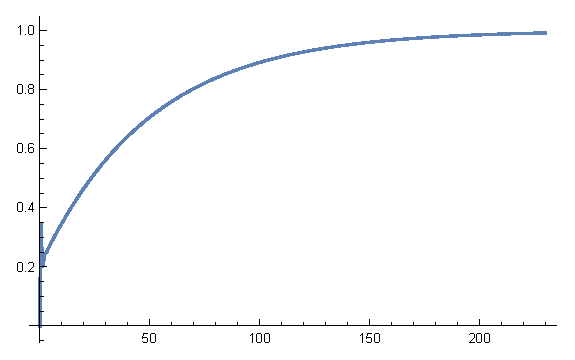
\includegraphics{pset1_gr1.eps}

\begin{doublespace}
\noindent\(\pmb{\text{FindRoot}[y[t]\text{==}0.99,\{t,230\}]}\)
\end{doublespace}

\begin{doublespace}
\noindent\(\{t\to 218.847\, -\text{3.5605271890862875$\grave{ }$*${}^{\wedge}$-61} i\}\)
\end{doublespace}

\end{document}
